%---------------------------
%	PREAMBLE
%---------------------------

\documentclass{article}

\usepackage[english]{babel}
\usepackage[utf8]{inputenc}
\usepackage{fourier}
\usepackage{fancyhdr}
\usepackage[parfill]{parskip}
\usepackage{hyperref}
\usepackage{graphicx}
\usepackage{float}
\usepackage{listings}
\usepackage{fourier}
\usepackage{tikz}
\usetikzlibrary{shapes.geometric, arrows}
\usepackage{textcomp}

\newcommand{\forceindent}{\leavevmode{\parindent=2em\indent}}

%------------------------%------------------------%

\begin{document}

\pagestyle{fancy}
\fancyhf{}
\rhead{Doing Survey Research \the\year}
\lhead{https://github.com/Yuji-Shimohira-Calvo/DSR}
\rfoot{Page \thepage}

\section*{\hfil Lab Worksheet IX \hfil}
\subsection*{Multiple regression analysis}

In today's worksheet we are going to do some multiple regression analysis on respondents' self-reported happiness using the \textit{European Social Survey}. You can find the dataset \textbf{essuk16.dta} on LEARN. Since it is the same dataset we used in the previous worksheet, the same caveats established then also apply here (e.g., regression assumptions are not considered for simplicity's sake) . Remember three key Stata commands widely used to explore datasets:

\begin{lstlisting}
describe
summarize
codebook, compact
\end{lstlisting}

We should be paying attention to things like the number of variables in the dataset, what they measure, how they are coded, whether we have missing cases and how these are coded. Last time we focused on the variables ``happy'', ``trstprt'', ``trstplt'', and ``atchctr.'' This time let's try:

\begin{lstlisting}
tabulate agea
tabulate region
tabulate gender
\end{lstlisting}

From the first tabulation we can see that respondents' ages range from 15 to 94. The command \texttt{summarize} would have given us this information more easily:

\begin{lstlisting}
summarize agea
\end{lstlisting}

However, remember that tabulations are not always the best way to represent and explore data. Since ``agea'' is a continuous variable we could plot it in a histogram:

\begin{lstlisting}
histogram agea, frequency
\end{lstlisting}

Also, you can explore two variables at the same time using the command \texttt{histogram}. For example, we could plot the distribution of respondents' ages in each region:

\begin{lstlisting}
histogram agea, frequency by(region)
\end{lstlisting}

On the other hand, ``region'' is a categorical variable, so we could plot it with bars like this:

\begin{lstlisting}
graph bar (percent), over(region, label(angle(45)))
\end{lstlisting}

The variable ``gndr'' is also categorical; however if you try plotting it in a bar chart or pie chart you might find it redundant because the variable only has two categories. Perhaps it is more convenient representing ``gndr'' with a simple tabulation (but again, this is a matter of personal preference). Stata allows you to explore data in a myriad of ways. For instance, consider the following:

\begin{lstlisting}
table gndr, contents(freq mean agea) row
\end{lstlisting}

With the \texttt{table} command and the \texttt{contents} option we can explore gender and age at the same time. The tabulation above shows the mean (average) age for males and females. Tabulating means (not only frequencies or percentages) could sometimes be very useful. If you were to ask the data ``are males happier than females?'' you would probably want to start by looking at the average level of happiness:

\begin{lstlisting}
table gndr, contents(freq mean happy) row
\end{lstlisting}

and you would find that female respondents are ever so slightly happier than male respondents on average (7.66 versus 7.6).

Now that we have explored a few variables let's run some regressions. Start with:

\begin{lstlisting}
regress happy gndr agea ib7.region
\end{lstlisting}

\begin{figure}[H]
	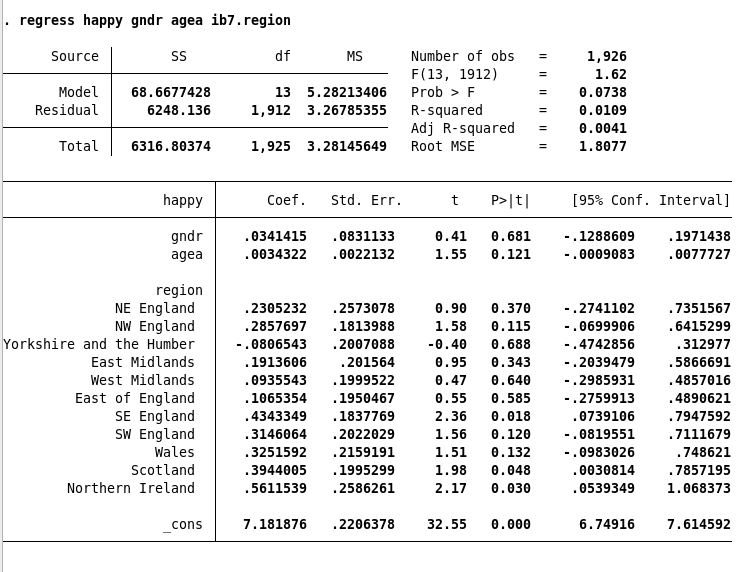
\includegraphics[width=\linewidth]{../img/mult_reg1.png}
	\caption{Multiple linear regression model with happiness as outcome.}
\end{figure}

Remember that linear regression requires continuous variables as your dependent variable. In the model above, variables ``happy'' and ``agea'' are considered continuous, whereas ``gndr'' and ``region'' are categorical. It is important to tell Stata that it needs to treat specific variables as categorical, for your model will need $X-1$ \textit{dummy variables} (where $X$ is the total number of categories in a variable). Take ``region'' as an example: this variables has twelve categories (twelve regions), therefore your model will need eleven dummy variables and one \textit{base group}. In the command above, Stata has been instructed to treat ``London'' as base group (\texttt{ib7.} does that, if you wanted the second category to be the base group instead, you can type \texttt{ib2.} before the variable name).

The value of $R^2$ tells you the proportion of variance in your dependent variable (``happy'') that is explained by the model. In this case, we can see that this model does not really explain much, only 1.1 percent of variance or information. Moreover, if we look at the $p$-value for the $F$-test of overall significance (reported as $Prob > F$ in Stata) we can see that it is not statistically significant itself. This is telling us that our model does not fit any better than a model with no predictors (also called \textit{intercept-only}). 

Most coefficients are not statistically significant at the 0.05 level (we already knew this from the $F$-test of overall significance). A non-statistically significant coefficient is telling you that we cannot be sure the coefficient (i.e., the value of the parameter) is actually different from zero. If you look at the confidence interval of a non-statistically significant coefficient, you will see that the interval includes zero in its range. This means you should not interpret that coefficient. However, do acknowledge in your papers and reports that you have non-statistically significant coefficients by simply saying so.

Let's now run the following regression model:

\begin{lstlisting}
regress atcherp gndr agea ib7.region
\end{lstlisting}

Notice that this new model loses 16 observations (not many) when compared to our previous ``happiness model'' (the observations go from 1,926 to 1,910). However, now our $F$-test is statistically significant  ($Prob > F = 0.0000$), meaning that our model fits better than an empty or intercept-only model. The model explains about 2.8 percent of information in the dependent variable ``atcherp'' (a 0-to-10 scale of emotional attachment to Europe).

It is of \underline{paramount importance} to bear in mind that the interpretation of coefficients of categorical variables is \underline{totally different} from the interpretation of coefficients of continuous variables. Below the coefficients of the variables ``agea'' (continuous) and ``gndr'' (categorical) are interpreted for you:

\begin{itemize}
	\item ``agea'': keeping the rest of variables constant, for each one-unit increase in a respondent's age we expect a decrease of 0.01 points in emotional attachment to Europe.
	\item ``gndr'': keeping the rest of variables constant, female respondents present an emotional attachment to Europe 0.281 points higher than that of male respondents. 
\end{itemize}

\begin{figure}[H]
	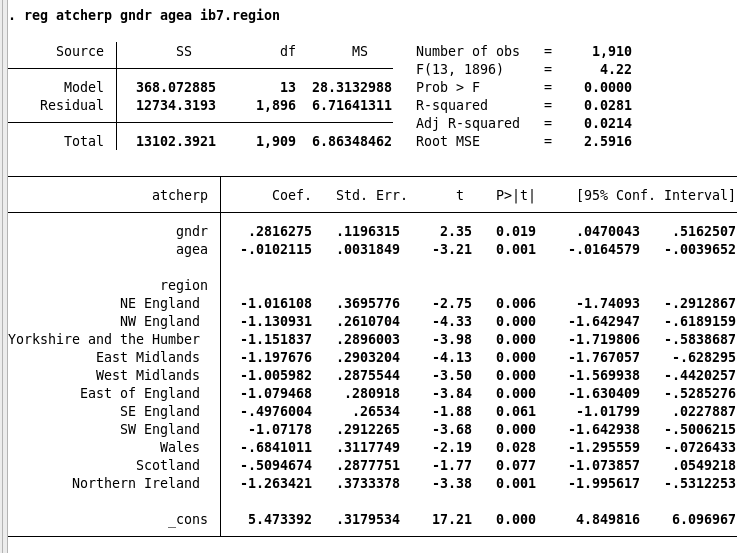
\includegraphics[width=\linewidth]{../img/mult_reg2.png}
	\caption{Multiple linear regression model with emotional attachment to Europe as outcome.}
\end{figure}

Firstly, notice that when interpreting regression coefficients in multiple regression \textit{you must} keep constant the variables you are not interpreting. Secondly, when interpreting continuous variables we speak of ``one-unit increase'' if the coefficient is positive or of ``one-unit decrease'' if the coefficient is negative. However, when interpreting categorical variables (dummy variables) we compare groups to the base group. In the example above, there are only two categories: males and females. Because the variable is coded 1 "male'' and 2 ``female'', Stata takes by default the first value, ``male'', as base group. The coefficient of ``gndr'', therefore, is really the coefficient of female respondents in comparison to that of male respondents. Here too a positive coefficient means an increase, but it is an increase over the base group's effect on the dependent variable. To clarify this point further consider the variable ``region'' below (remember the base group was ``London''):

\begin{itemize}
	\item ``NE England'': keeping the rest of variables constant, respondents from the North East (England) are 1 point less emotionally attached to Europe than respondents from London.
	\item ``Scotland'': keeping the rest of variables constant, respondents from Scotland are 0.51 points less emotionally attached to Europe than respondents from London.
\end{itemize}

Because all regional categories (i.e., all the dummy variables in the model) present a negative coefficient, we know that London is the region most emotionally attached to Europe. The interpretation of all these coefficients will therefore be in ``negative'' terms (less than the base group). Needless to say that if we did not know that ``London'' is the base group we could not interpret these figures. Also, notice that Scotland's coefficient is not statistically significant. What you already know about statistical significance also applies here in the same fashion: because $p > 0.05$ in the case of the category ``Scotland'', we cannot say for sure the coefficient is different for zero (and we do not interpret it). Finally, the closer the coefficient of a dummy variable is to zero the more similar that category is to the base group.   

\end{document}
